% Generated by paper/gen.py from paper/data. Do not edit.
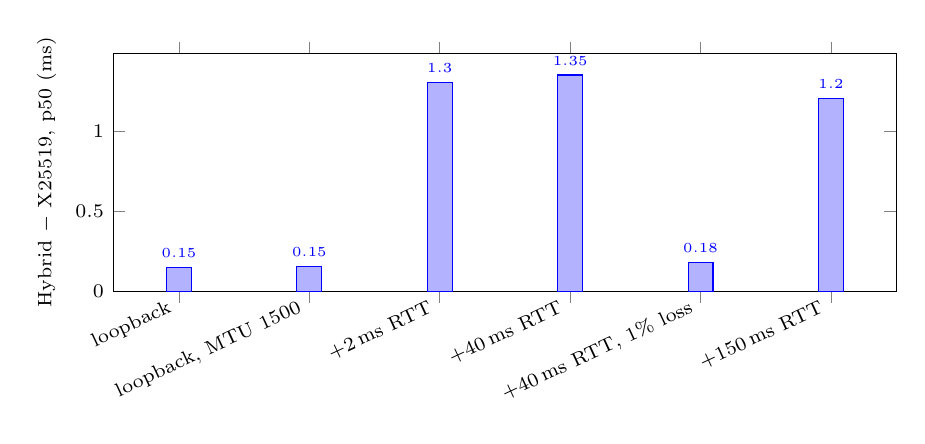
\begin{tikzpicture}
\begin{axis}[
  ybar, ymin=0, width=0.95\linewidth, height=4.6cm, bar width=9pt,
  symbolic x coords={{loopback},{loopback, MTU 1500},{+2\,ms RTT},{+40\,ms RTT},{+40\,ms RTT, 1\% loss},{+150\,ms RTT}}, xtick=data,
  x tick label style={font=\scriptsize, rotate=25, anchor=east},
  y tick label style={font=\scriptsize}, label style={font=\scriptsize},
  ylabel={Hybrid $-$ X25519, p50 (ms)},
  nodes near coords, every node near coord/.append style={font=\tiny, /pgf/number format/.cd, fixed, precision=2},
]
\addplot coordinates {({loopback},0.148) ({loopback, MTU 1500},0.154) ({+2\,ms RTT},1.303) ({+40\,ms RTT},1.349) ({+40\,ms RTT, 1\% loss},0.180) ({+150\,ms RTT},1.204)};
\end{axis}
\end{tikzpicture}
